\subsection{RBA}

\paragraph{Principe}

Le principe est expliqué dans \citet{goelzer_cell_2011} et est brièvement reproduit sur la \reffigt{fig:rba}. L'article contient les définitions et preuves du modèle.

\begin{figure}[ht]
  \centering
  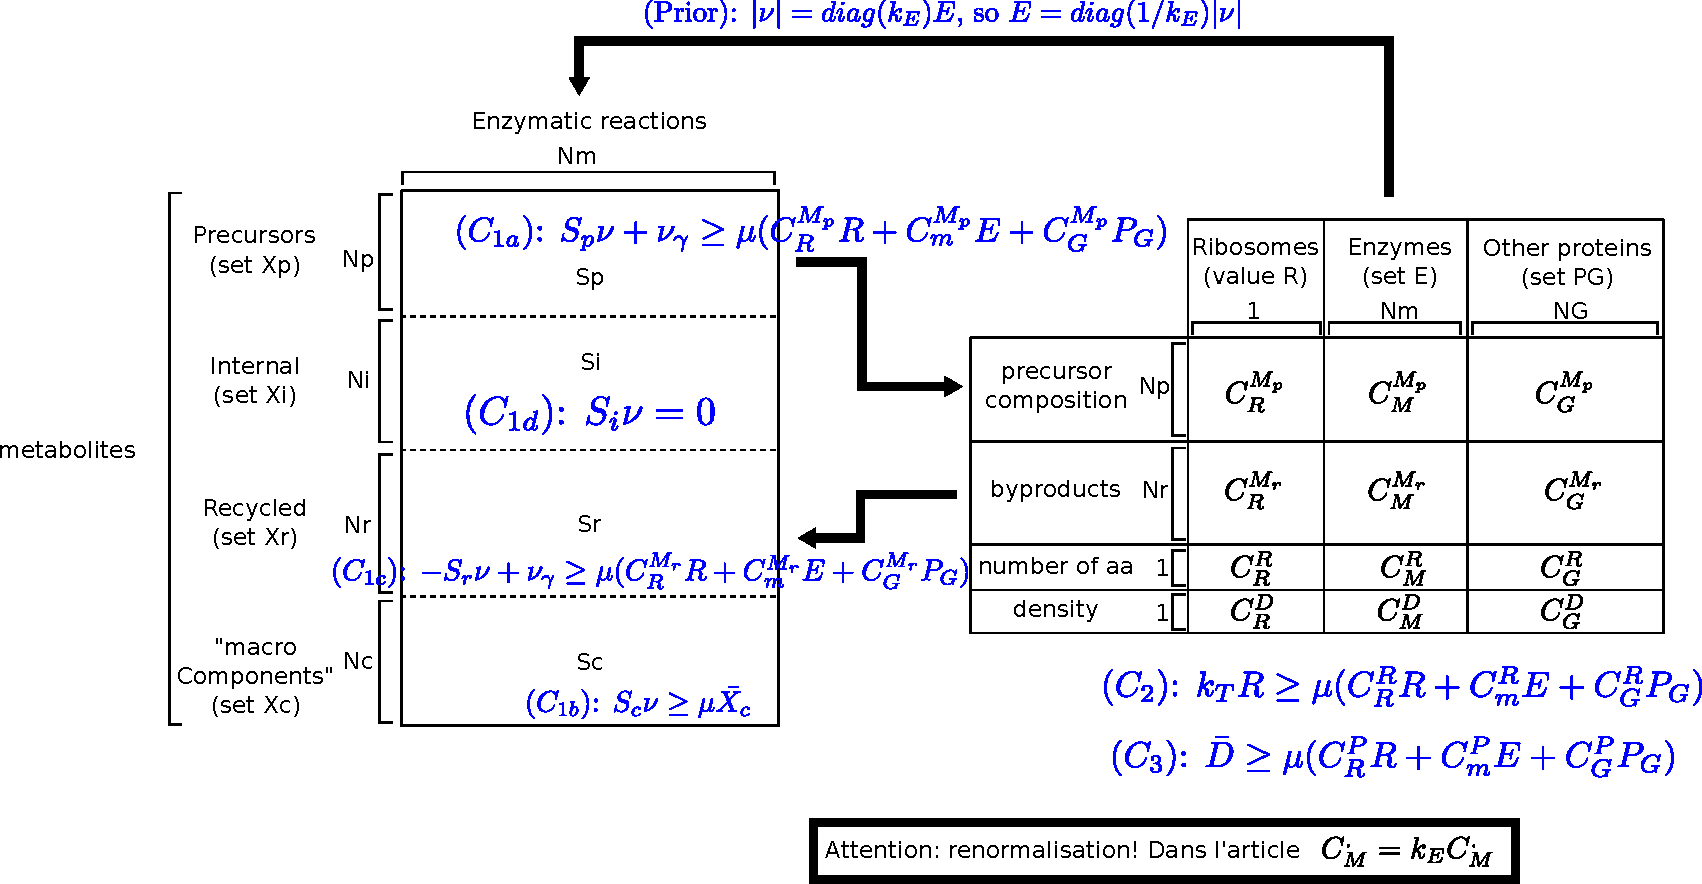
\includegraphics[width=\linewidth]{RBA}
  \caption{Schéma de fonctionnement des RBA.}
  \label{fig:rba}
\end{figure}

\paragraph{Formulation mathématique}

\paragraph{Interprétations mathématiques}

\paragraph{Applications}
\citet{goelzer_cell_2011} applique les RBA à la croissance chez \textit{B. subtilis}. Les cellules croissent dans un milieu qui varie de riche à pauvre. Plus le milieu est riche, plus les bactéries croissent rapidement. Le premier résultat positif est l'augmentation de la part de ribosome et la diminution de la part de protéines métaboliques dans le pool total des protéines. Les auteurs montrent mathématiquement que les RBA permettent de désactiver complètement un pathway à cause de la quantité de protéines nécessaires à maintenir des pathways alternatifs. Quand un a.a. est ajouté au milieu, on observe que sa synthèse \textit{de novo} cesse complètement (ou presque).

La solution des RBA fournit un jeu de régulations qui permettrait d'obtenir un taux de croissance optimal. On peut s'attendre à ce que ces régulations soient effectivement implémentées. D'après \citet{goelzer_cell_2011}, on a un assez bon accord entre prédictions et données. Un exemple avec un switch sur des transporteures à basse et haute affinités est donné pour fournir une illustration simple du phénomène.

Une analyse un peu différente est présentée dans \citet{goelzer_quantitative_2015}. Le but est d'estimer les répartitions globales des ressources chez \textit{B. subtilis}. Le modèle prend en compte le folding via l'introduction de chaperones (mathématiquement de la même façon que les ribosomes). Grâce à de nombreuses données, les efficacités enzymatiques sont estimées (elles étaient fixées de façon \textit{ad hoc} dans \citet{goelzer_cell_2011}). Cela permet de donner un coût en nombre de protéines aux différents sous-processus de la cellule. Une analyse de sensibilité montre que les paramètres liés à la répartition des protéines (densité, fraction de protéines cytosoliques, etc.). Dans le supplementary material, les auteurs montre que les résultats se recoupent partiellement avec une analyse FBA, mais les FBA échouent à allouer correctement les protéines. Globalement le modèle proposé est beaucoup plus riche que dans l'article précédent. J'ai raté beaucoup de subtilités il faudra que je revienne un peu dessus au fur et à mesure.
